% EV & BAT
\newglossaryentry{EV}{name={EV}, description={Electric Vehicle}}
\newglossaryentry{OBD-II}{name={OBD-II}, description={On-Board Diagnostic II}}
\newglossaryentry{SOC}{name={SOC}, description={State of Charge}}
\newglossaryentry{BMS}{name={BMS}, description={Battery Management System}}
\newglossaryentry{SOH}{name={SOH}, description={State of Health}}
\newglossaryentry{NMC}{name={NMC}, description={lithium nickel manganese cobalt oxide (LiNiMnGoO\textsubscript{2})}}
\newglossaryentry{IoT}{name={IoT}, description={Internet of Things}}
\newglossaryentry{ECU}{name={ECU}, description={Electronic Control Unit}}
\newglossaryentry{ECO}{name={ECO}, description={Economy Mode}}
\newglossaryentry{GPS}{name={GPS}, description={Global Positioning System}}
\newglossaryentry{HV}{name={HV}, description={High Voltage}}
\newglossaryentry{BEV}{name={BEV}, description={Battery Electric Vehicle}}


% AI
\newglossaryentry{SVR}{name={SVR}, description={Support Vector Regression}}
\newglossaryentry{CNN}{name={CNN}, description={Convolutional Neural Network}}
\newglossaryentry{MLP}{name={MLP}, description={Multilayer Perceptron}}
\newglossaryentry{ML}{name={ML}, description={Machine Learning}}
\newglossaryentry{ANN}{name={ANN}, description={Artificial Neural Network}}
\newglossaryentry{LSTM}{name={LSTM}, description={Long Short-Term Memory}}
\newglossaryentry{Bi-LSTM}{name={Bi-LSTM}, description={Bidirectional Long Short-Term Memory}}
\newglossaryentry{AI}{name={AI}, description={Artificial Intelligence}}
\newglossaryentry{FC}{name={FC}, description={Fully Connected}}
\newglossaryentry{RL}{name={RL}, description={Reinforcement Learning}}
\newglossaryentry{MSE}{name={MSE}, description={Mean Squared Error}}
\newglossaryentry{RMSE}{name={RMSE}, description={Root Mean Squared Error}}
\newglossaryentry{MAE}{name={MAE}, description={Mean Absolute Error}}

\chapter{Electrified Motion: Driving Patterns, Energy Use, and Thermal Dynamics in EV Batteries}\label{ch:5}
\minitoc

Understanding the impact of driving behavior on battery thermal dynamics is essential for enhancing \gls{EV} performance and longevity. 
This chapter investigates the influence of driving patterns on battery temperature and power consumption using a comprehensive dataset from a \textit{Nissan Leaf} 2018 Acenta. 
A \gls{Bi-LSTM} model predicts battery temperature, offering valuable insights for optimizing thermal management and preserving battery health.

\newpage

\section{Battery Structure and Internet of Things Device}
\label{sec:thermal_dynamics_case_study_intro}

The \gls{EV} battery is a 40 kWh lithium-ion pack shows in Figure~\ref{fig:leaf_bat_pack} (uses \gls{NMC} laminate cells~\cite{calearo2019modeling}) with 192 cells arranged in 24 modules. 
The cathode and anode are respectively made of graphite and $Li[Ni_xMn_yCo_z]O2$. 
An \gls{IoT} sensor in Figure~\ref{fig:colletion_setup} that was self-developed (collaborated with the University of Bologna~\cite{CCNC_2022}) has been collecting data from the \glspl{ECU} through \gls{OBD-II} port since year 2021. 

%Appendices~\ref{append:data_result} and \ref{append:tech_detail} include the initial data and \gls{IoT} sensor architecture, respectively.

\begin{figure} [htbp]
	\centering
	\begin{subfigure}{0.45\linewidth}
		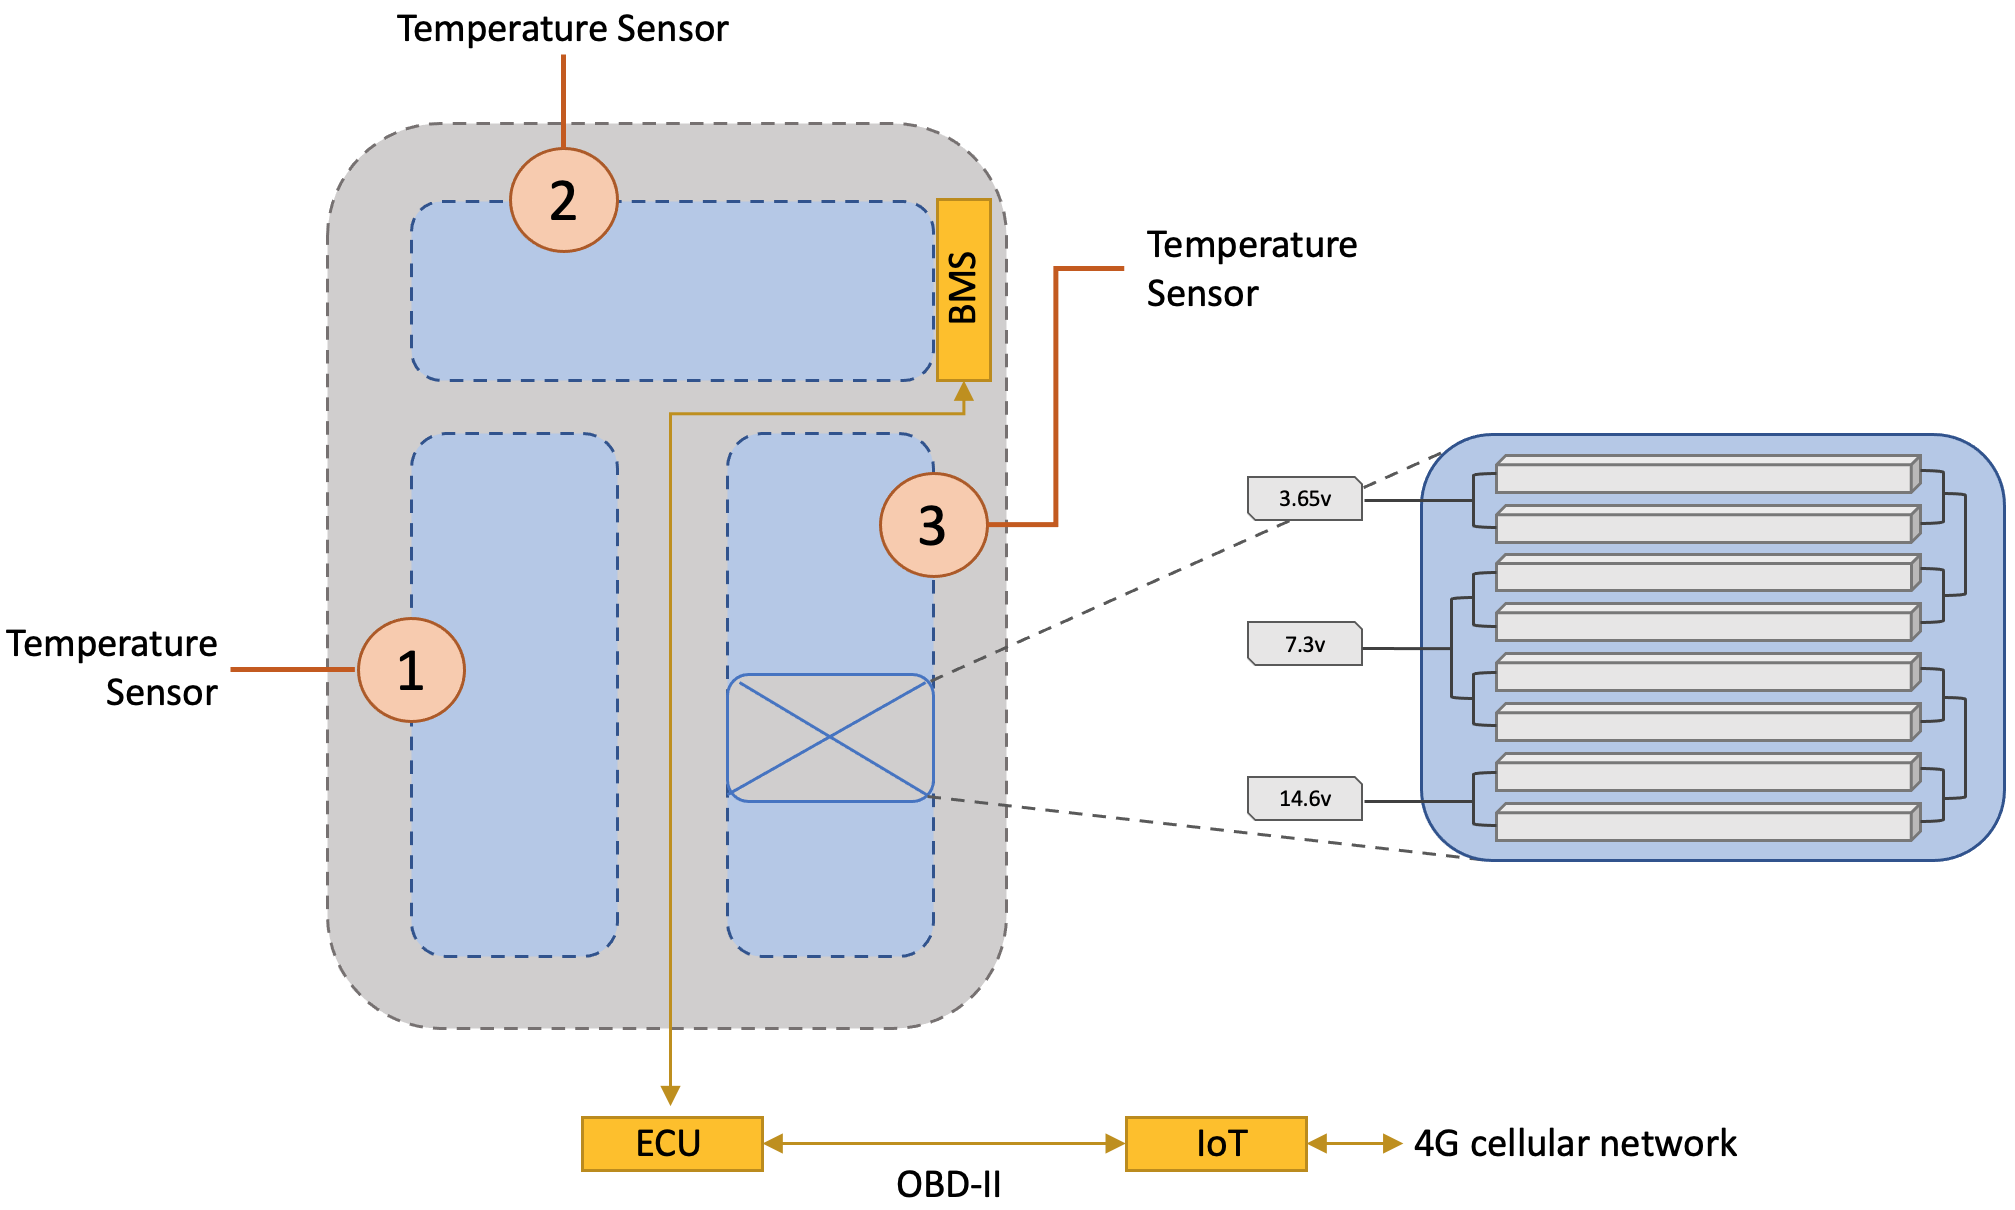
\includegraphics[width=\linewidth]{Chapter5/figures/leaf_pack_temp_sensor.png}
		\caption{\textit{Nissan Leaf} battery structure~\cite{kane_2020_see}}
        \label{fig:leaf_bat_pack}
	\end{subfigure}
	\quad
    \begin{subfigure}{0.42\linewidth}
		\includegraphics[width=\linewidth]{Chapter5/figures/obdii.png}
		\caption{4G cellular \gls{IoT} with \gls{OBD-II} port}
        \label{fig:colletion_setup}
	\end{subfigure}
    \caption{Data collection setup}
\end{figure}

\section{Dataset and Data Collection}

The dataset with driver's label comprises over 4.5 million samples, recorded at a temporal resolution of 250 milliseconds, spanning 7,100 kilometers of real-world driving in 384 days. 
Key recorded parameters include:

\begin{itemize}
    \item \textbf{Battery Metrics:} Voltage, current, pack temperature, \gls{SOH}, and \gls{SOC}.
    \item \textbf{Driving Behavior:} Acceleration, braking pedal pressure, and speed.
    \item \textbf{Environmental Factors:} Ambient temperature, weather conditions, and seasonal variations.
\end{itemize}

The dataset captures diverse driving styles from drivers with anonymous processed, environmental conditions, and road types, enabling a detailed analysis of how external and behavioral factors influence battery temperature.
The total distance traveled and battery's \gls{SOH} are shown in Figure~\ref{fig:soh_odometer}. 
The \gls{SOH} unexpectedly shows a loss of about 1.5\% from July to September and 1\% in the single month of November 2021. 
However, the odometer grows linearly. 
Several factors, including charging (slow, regular, and quick charge), temperature, acceleration, and driving conditions can possibly cause the drop of the battery health. 

\begin{figure}[htbp]
    \centering
	\begin{subfigure}{0.47\linewidth}
        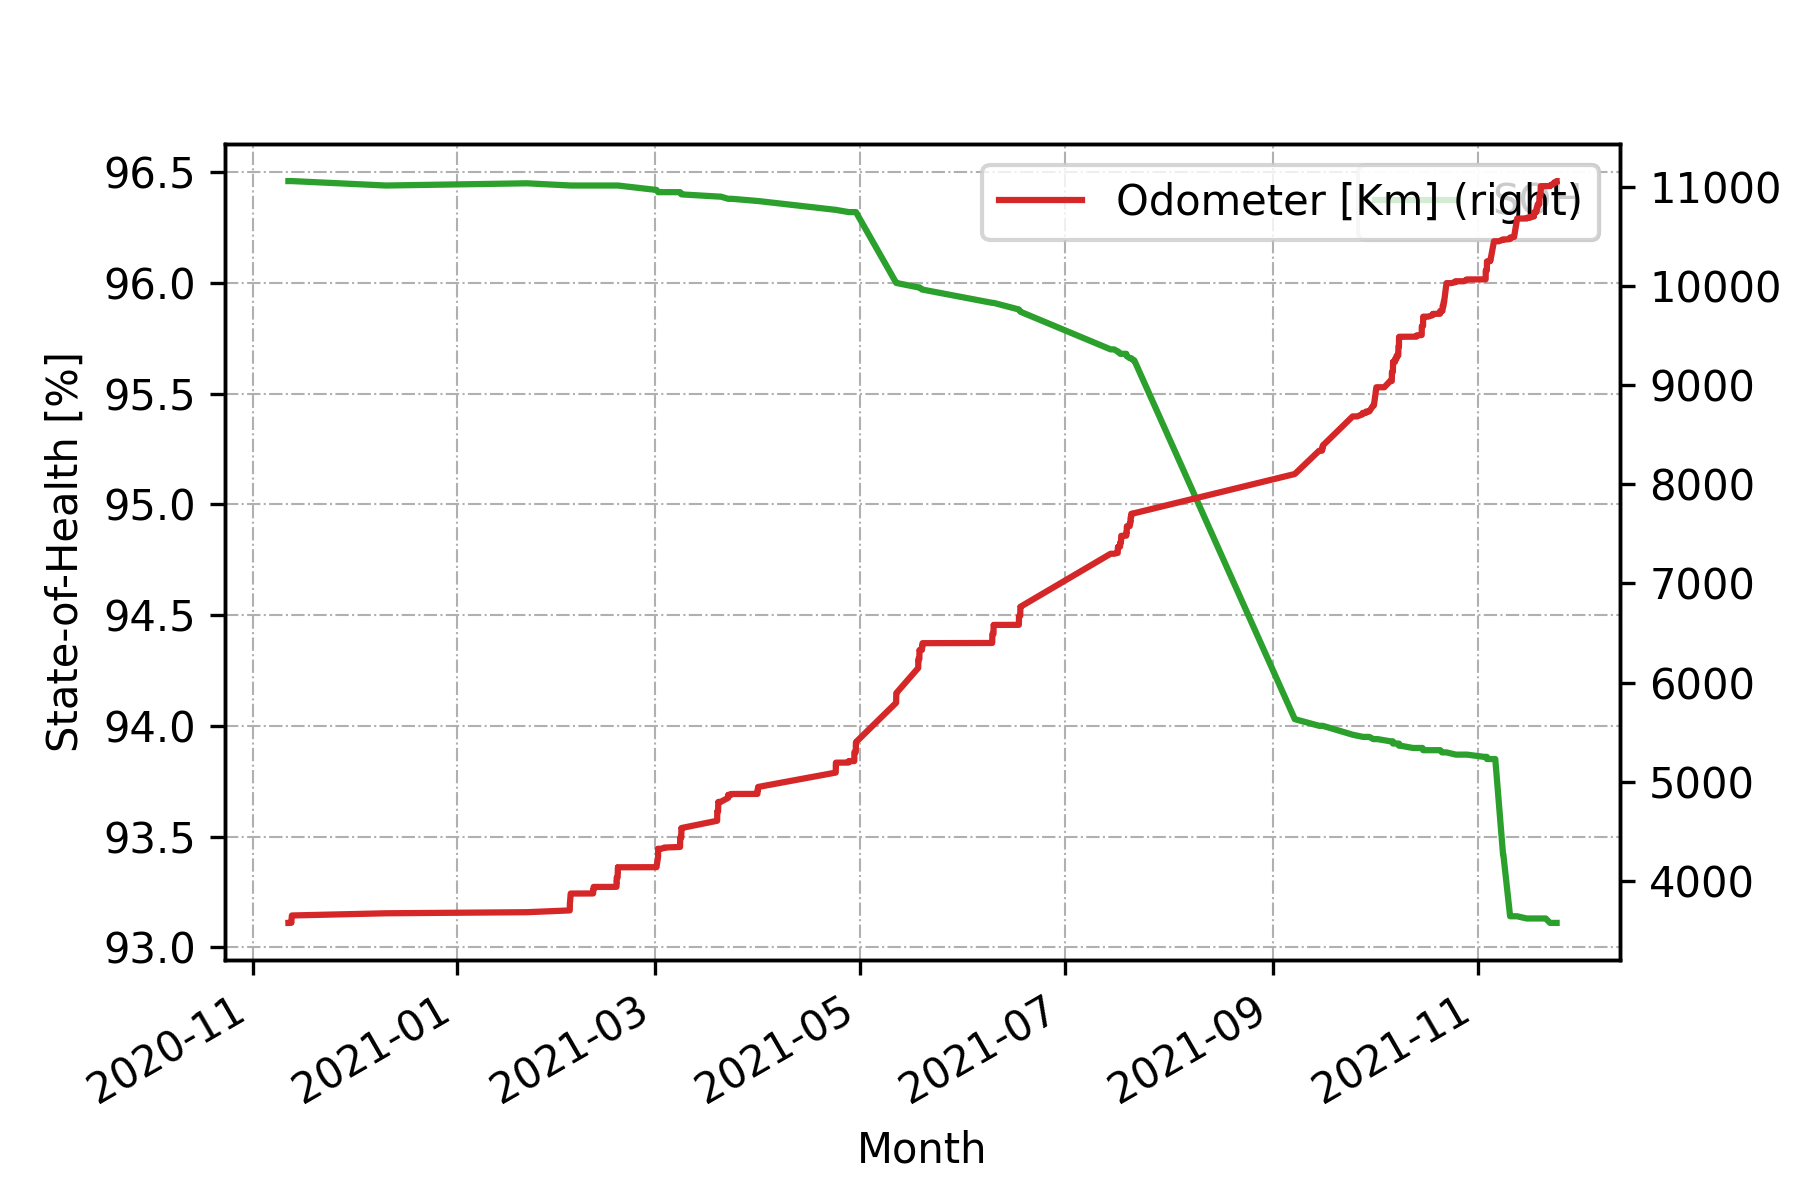
\includegraphics[width=\textwidth]{Chapter5/figures/ch5_SOH_Odometer_colored.png} 
        \caption{State of Health and driving distance of the dataset}
        \label{fig:soh_odometer}
	\end{subfigure}
    \quad
    \begin{subfigure}{0.43\linewidth}
        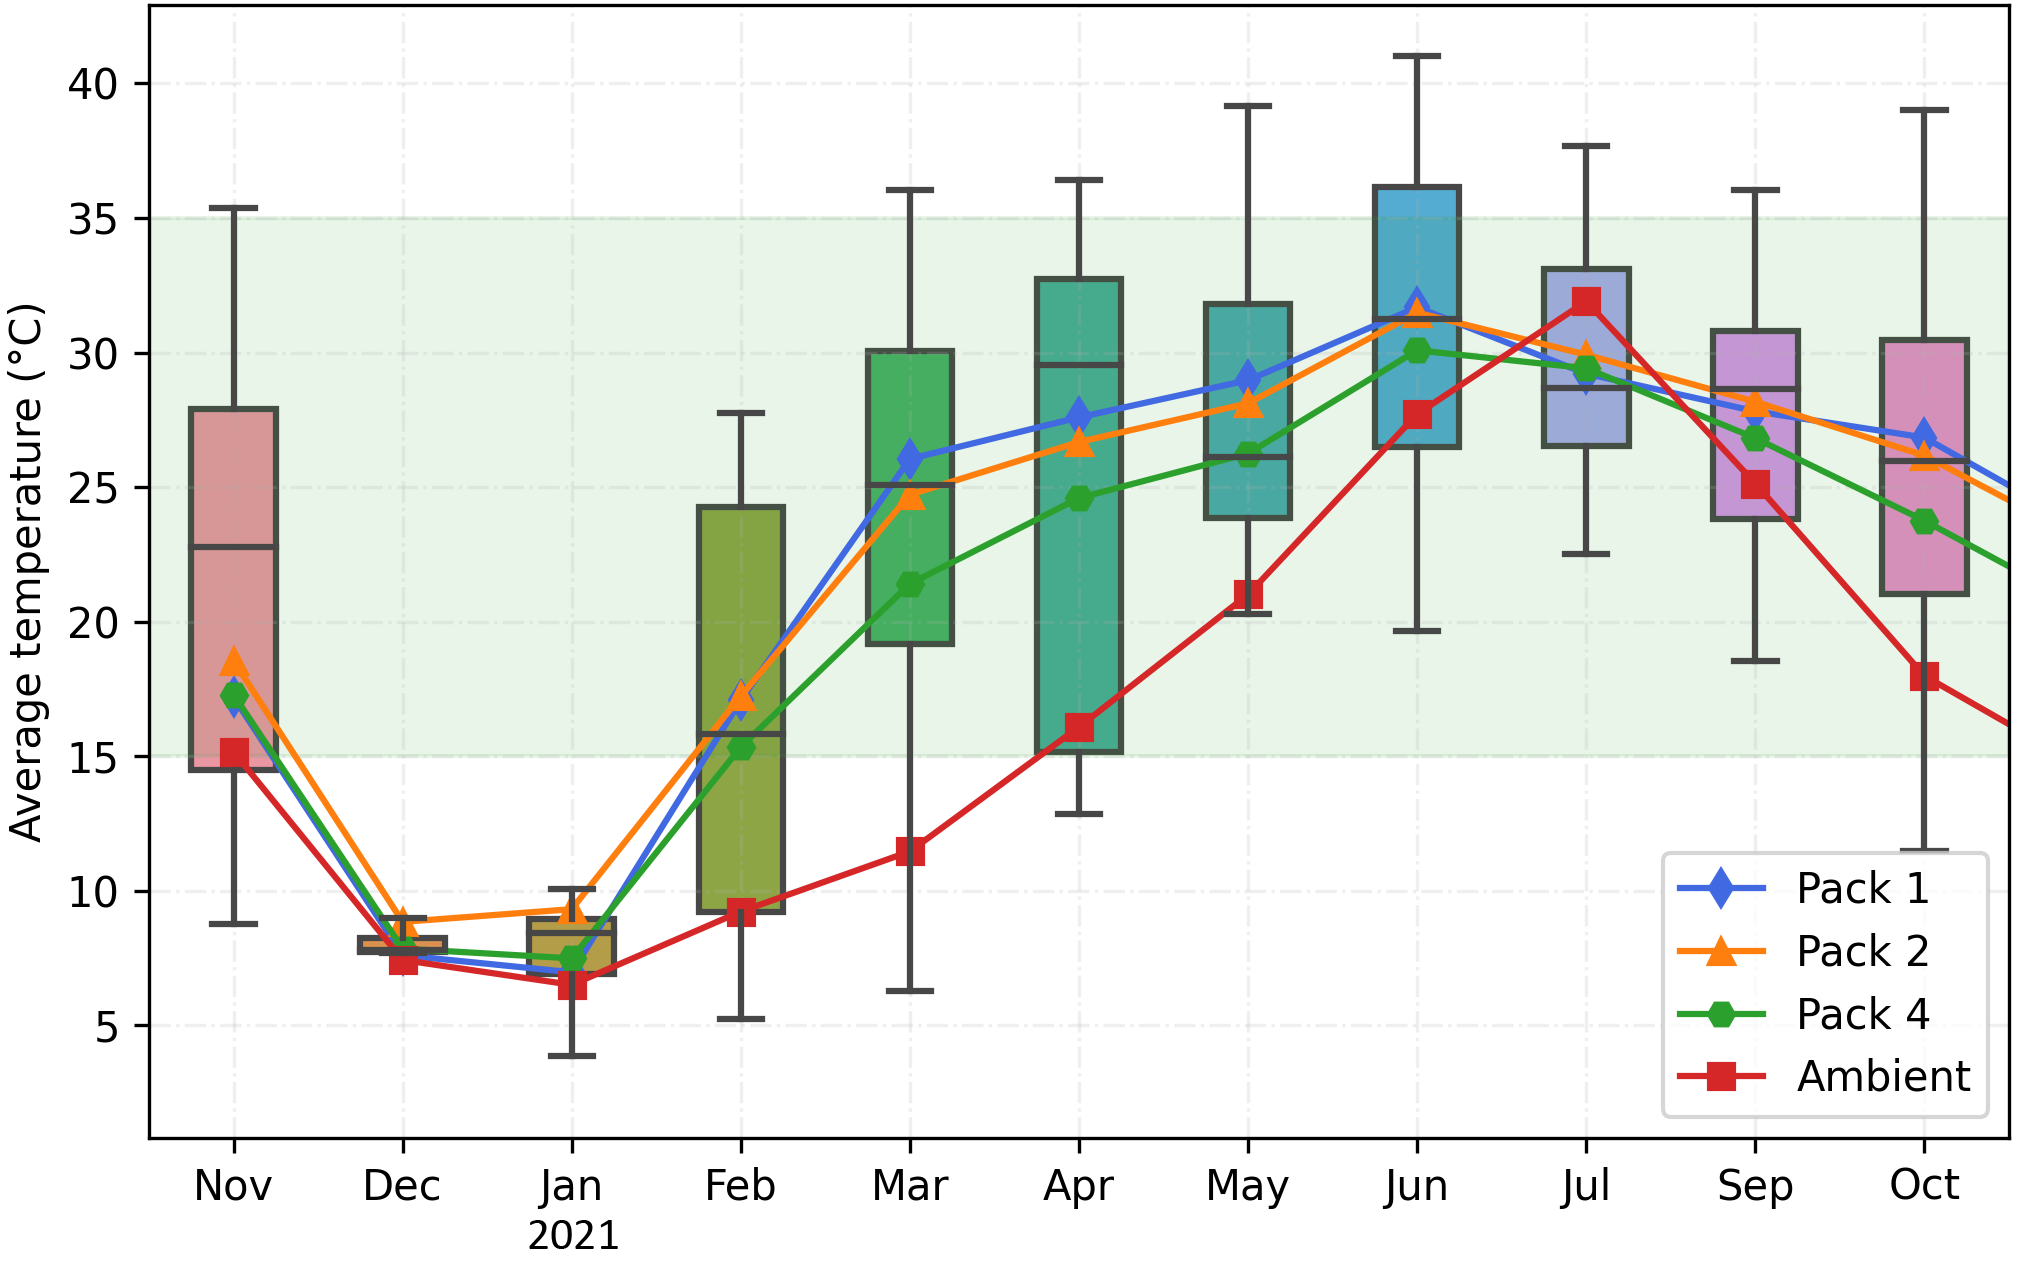
\includegraphics[width=0.9\textwidth]{Chapter5/figures/BAT_SEASONAL_PACK_MEAN.png}
        \caption{Temperature of all packs. The green area corresponds to the optimal range. Leaf 40kWh lacks pack \#3.}
        \label{fig:avg_pack_temp}
	\end{subfigure}
    \\
    \begin{subfigure}{0.45\linewidth}
        \includegraphics[width=\linewidth]{Chapter5/figures/thermal_A4-cropped_cropTemp.pdf}
        \caption{Seasonal battery temperature}
        \label{fig:seasonal_temp}
    \end{subfigure}
    \quad
    \begin{subfigure}{0.45\linewidth}
        \includegraphics[width=\linewidth]{Chapter5/figures/thermal_A4-cropped_cropGPS.pdf}
        \caption{Battery pack temperature in location}
        \label{fig:pack_location_temp}
    \end{subfigure}
    \caption{State of Health and battery pack temperature from the collected period}
    \label{fig:expanded_setup}
\end{figure}

Four individual temperature sensors are on the Leaf's pack. 
Figure~\ref{fig:avg_pack_temp} shows the average temperature status from the individual sub-battery packs monthly. 
Rectangles represent the \gls{HV} battery temperature while single packs' average temperature are shown with lines. 
This is the overall status that includes the driving, charging, and idling phases. 
Depending on the pack's location, the data shows that the temperature difference is 2°C to 5°C on a monthly average. 
Most of the time, the battery pack can stay at the optimal temperature range (under 35°C and higher than 15°C).

The seasonal variation in Italy reveals that battery temperatures are typically higher in summer due to increased ambient heat, 
while winter temperatures are significantly cooler, reflecting the expected climate patterns of hot summers and cold winters, as shown in Figure~\ref{fig:seasonal_temp}.
Battery temperature also fluctuates based on location: 
in traffic or low-speed areas, reduced airflow and sustained loads cause overheating, 
while on highways, elevated temperatures result from the high current output required for acceleration and maintaining speed, as shown in Figure~\ref{fig:pack_location_temp}.
Additionally, as shown in Figure~\ref{fig:pack_location_temp}, 
the battery remains hot after transitioning from highways or high-speed areas to low-speed areas, as it requires time to cool down due to residual thermal inertia.


\section{Data Preprocessing and Feature Engineering}

The dataset underwent comprehensive preprocessing to extract relevant features and normalize the data for subsequent analysis and model training. 
Due to the nature of \gls{OBD-II} raw data, which is recorded at intervals as short as 250 milliseconds, the dataset is inherently noisy. 
This high-frequency sampling results in the capture of transient anomalies and extreme outliers that do not accurately reflect the true operating conditions of the vehicle. 
Consequently, filtering is essential to ensure the reliability of the analysis.

\subsection{Data Preprocessing}

To address this, the data was filtered according to specific criteria, as outlined in Table~\ref{tab:filtering_criteria}. 
These criteria were designed to remove impossible or unrealistic values, such as negative speeds, unreasonably high battery temperatures, or inconsistencies in odometer readings. 
Without this initial filtering step, the noise in the dataset would dominate, rendering subsequent statistical techniques, such as z-score filtering or standardization, ineffective in isolating meaningful patterns. 
This is because extreme outliers can distort the normalization process, particularly when they occur at such high frequencies.

After filtering for impossibilities, a moving average was applied to variables prone to rapid fluctuations, such as odometer readings and battery pack temperatures. 
This step smooths out short-term variations and provides a clearer representation of long-term trends. 
By reducing the impact of noise and outliers, this preprocessing framework ensures that the dataset is better suited for accurate modeling and interpretation, ultimately enhancing the quality and robustness of the analytical outcomes.

\begin{table}[!ht]
    \begin{center}
    \caption{Range Specification for Data Filtering Criteria}
    \label{tab:filtering_criteria}
    \begin{tabular}{llcl}
    \toprule
    \multicolumn{4}{c}{Driving} \\ 
    Variables & Interval [s] & Range & Unit \\ 
    \midrule
    Odometer & 10 & $0 < x < 100,000$ & Km \\ 
    Timestamp & 0.25 & ~ & Microseconds \\ 
    Power\_SW & 100 & $0/1$ & - \\ 
    Lat & 1 &$42-48$ & $^\circ$ \\ 
    Long & 1 & $11.2 - 13.3$ & $^\circ$ \\ 
    Speed & 1 & $0 < x < 160$ & Km/h \\ 
    Gear & 100 & $0-4$ & - \\ 
    RangeKm & 10 & $0$ to $300$  & Km \\ 
    RPM & 0.25 & $0 - 18,000$ & Rev/min \\ 
    SOC & 0.25 & $0-100$ & \% \\ 
    SOH & - & $99 - 80$ & \% \\ 
    Torque & 1 & $0$ to $400$ & Nm \\ 
    Motor\_Temp & 10 & $0-120$ & $^\circ$C \\ 
    Rain\_level & - & $1-4$ & - \\ 
    TP\_FR/TP\_FL/TP\_RR/TP\_RL & - & $200$ to $300$ & kPa \\ 
    Aux\_Pwr\_100W & 10 &  $0-1,000$ & W \\ 
    AC\_Pwr\_250W & 10 & $-3k-3k$ & W \\ 
    HV\_Bat\_Voltage & 0.25 & $300$ to $450$ & V \\ 
    HV\_Bat\_Current\_2 & 0.25 & $-400$ to $200$ & A \\ 
    HeaterTemp & 100 & $16.5$ to $30$ & $^\circ$C \\ 
    FanSpeed & 100 & $0$ to $8$ & - \\ 
    Brake & 1 & $0$ to $200$  & - \\ 
    Acc\_Pedal & 1 & - & - \\ 
    ECO & 10 & $0/1$ & - \\ 
    ePeda & 10 & $0/1$ & - \\ 
    Ambient\_C\_Temp & 10 & $-7 < x < 50$ & $^\circ$C \\ 
    Pack\_1\_C\_Temp & 60 & $0$ to $65$ & $^\circ$C \\ 
    Pack\_2\_C\_Temp & 60 & $0$ to $65$ & $^\circ$C \\ 
    Pack\_4\_C\_Temp & 60 & $0$ to $65$ & $^\circ$C \\ 
    \midrule
    \multicolumn{4}{c}{Charging} \\ 
    Variables & Range & Unit \\ 
    \midrule
    Plug\_State & 100 & $0-2$ & - \\ 
    Charge\_Mode & 100 & $0-3$ & - \\ 
    Quick\_Charge & - & $>0$ & - \\ 
    L1\_L2\_Charge & - & $>0$ & - \\ 
    HV\_Bat\_Voltage & 0.25 & $300$ to $450$ & V \\ 
    HV\_Bat\_Current\_2 & 0.25 & $-50 < x <200$ & A \\ 
    \bottomrule
    \end{tabular}
    \end{center}
    \footnotesize{
        \textbf{Remark:} If the 'Interval [s]' value is '-', it indicates that the variable is either updated only once at vehicle startup or not observed.
        The dataset comprises 7.3 million rows spanning from January 21, 2021, to July 29, 2022, covering a period of 554 days after filtering which is the extension on \cite{CCNC_2023}.
        Features containing defects or unrelated to the HV Battery are excluded from the this dataset.
    }

\end{table}

The \href{https://drive.google.com/drive/folders/1kWsFL2bpmckD-Muj2zxcFtk2Ac_ZPdUg?usp=sharing}{dataset with drivers' label}, was preprocessed following a systematic series of steps to prepare it for analysis. 
First, the raw discharge data from the test vehicle was selected for the period spanning from January 9, 2020, to August 3, 2022, encompassing approximately 2.4 million rows (equivalent to 168 hours of data). 
Next, additional calculations were performed to derive indirect variables for each record, including instant power, charging power, remaining power, acceleration, and horsepower. 
Subsequently, the data was analyzed to identify and label different groups of trips, accounting for variations in stopping intervals or different drivers on the same day. 
This process involved clustering and labeling individual trips, focusing on key events such as the activation of the vehicle's power-on button, changes in the charging plug state, and the charging mode. For consistency, a trip was defined as a sequence of records lasting more than 30 minutes.

To enhance data relevance, all features unrelated to driver behavior or the \gls{HV} battery output were excluded. 
Features powered by the 12V battery, such as headlights, fan speed, and wipers, were disregarded, as they do not directly contribute to the analysis of the HV battery's performance. 
This rigorous preprocessing approach ensured that the dataset was both relevant and optimized for subsequent analyses.
    
Figure~\ref{fig:intepo} shows the interpolation of the battery pack temperature in a trip. 
The bidirectional linear interpolation is applied to address the missing and null values. 
Trip-based z-score filtering is adopted to filter out the out-liners. 
For any values in a feature, the z-score larger than 3 (covered 99\% of the data) is set to null and interpolated. 
Any other abnormal values are interpolated if we identified any. 
The general summary of the high-quality discharge dataset ($\sim$130 hours) for the machine learning task is shown in Table~\ref{tab:the_dataset_overview}. 

\begin{figure}[ht]%[!ht]
    \begin {center}
    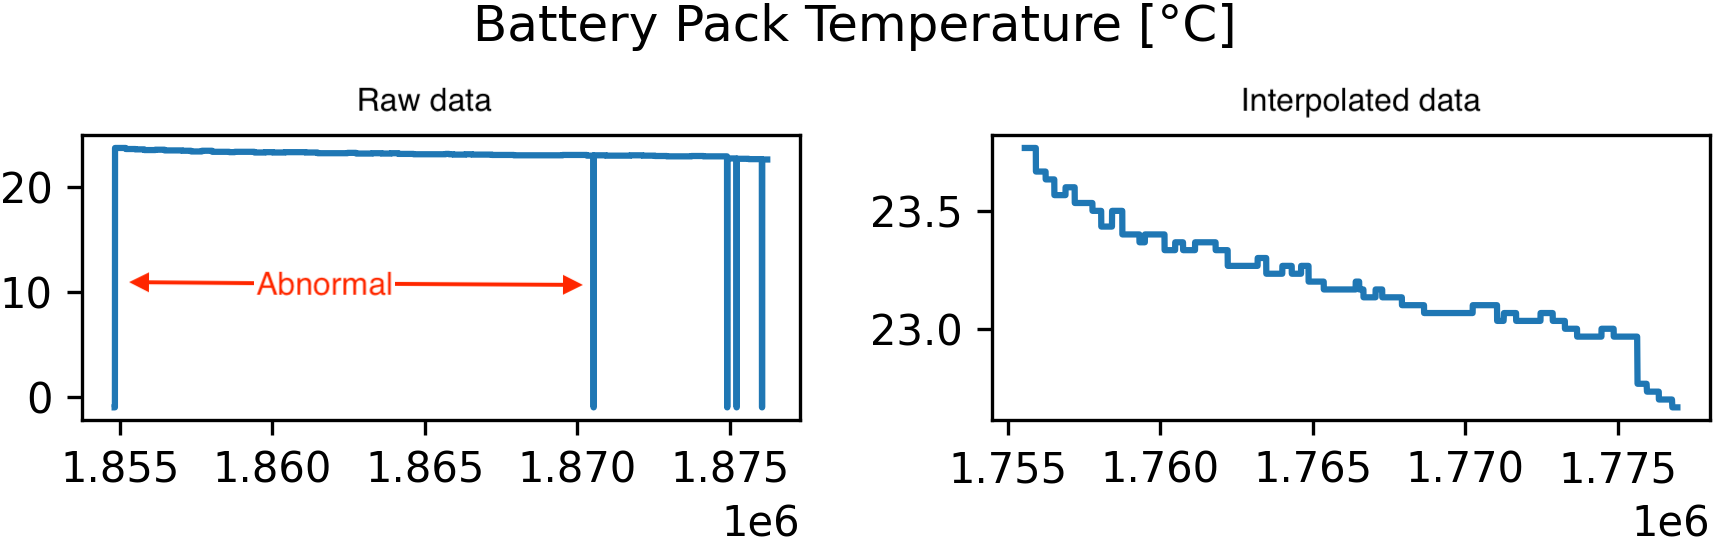
\includegraphics[width=1\textwidth]{Chapter5/figures/interpolated_temp.png}
    \caption{The bidirectional linear interpolation of null and missing values}
    \label{fig:intepo}
    \end {center}
\end{figure}

\begin{sidewaystable} % Rotates the table 90 degrees to the right
    \centering
    \begin{longtable}{lcccccccccc}
        \caption{The summary of filtered discharging dataset} \label{tab:the_dataset_overview} \\
        \toprule
        & Odometer & SOC & SOH & Voltage & Current* & Ambient °C 
        & Pack 1 °C & Pack 2 °C & Pack 4 °C & All Packs Avg. °C \\ 
        \midrule
        \endfirsthead
        \toprule
        & Odometer & SOC & SOH & Voltage & Current* & Ambient °C 
        & Pack 1 °C & Pack 2 °C & Pack 4 °C & All Packs Avg. °C \\ 
        \midrule
        \endhead
        \midrule
        \multicolumn{11}{r}{\textit{Continued on next page}} \\
        \midrule
        \endfoot
        \bottomrule
        \endlastfoot
        count & 1918299 & 1918299 & 1918299 & 1918299 & 1918299 & 1918299 
              & 1918299 & 1918299 & 1918299 & 1918299 \\ 
        mean & 9217.46 & 74.72 & 94.41 & 373.31 & -22.47 & 18.65 
             & 24.95 & 24.87 & 23.34 & 24.39 \\ 
        std & 3213.64 & 19.16 & 1.38 & 19.68 & 38.49 & 8.29 
            & 9.14 & 8.82 & 8.11 & 8.66 \\ 
        min & 255 & 0.32 & 92.63 & 0 & -370.67 & 3.5 
            & 5.8 & 5.6 & 5.76 & 5.83 \\ 
        25\% & 6673 & 61.2 & 93.06 & 356.13 & -39.22 & 12 
             & 17.3 & 17.45 & 16.4 & 17.1 \\ 
        50\% & 9431 & 78.99 & 93.91 & 374.95 & -5.59 & 17 
             & 25.2 & 25.1 & 23.3 & 24.7 \\ 
        75\% & 11890 & 91.39 & 95.88 & 391.41 & -0.98 & 24 
             & 32 & 31.44 & 29.44 & 30.97 \\ 
        max & 15537 & 99.11 & 96.46 & 655.35 & 179.66 & 44.5 
            & 55 & 54 & 48.4 & 52.47 \\ 
        Interpolated [\%] & 3.52 & 1.31 & 0.79 & 0.05 & 0.05 & 0 
                          & 0.02 & 0.02 & 0.02 & 0.02 \\ 
    \end{longtable}
    
    \begin{threeparttable}
        \begin{tablenotes}
            \item * The current load is negative when discharging (driving) and positive when regenerative braking.
        \end{tablenotes}
    \end{threeparttable}
    \end{sidewaystable}



\subsection{Feature Engineering}

\subsubsection{Data resampling}

certain driving-related factors are accumulated due to the long sampling rate on the battery pack's temperature. 
The fastest temperature sampling rate is about 60 to 90 seconds after the test on the \textit{Nissan Leaf}. 
If the 250 ms data is input directly to the \gls{ML} algorithms, it will cause a non-effective prediction of the results. 
This means the loss of the \gls{ML} models would be low, which is repeating the same output values but not effectively predicting the minor changes in the temperature. 
Figure~\ref{fig:temp_sample} shows a one-minute resample of the data. 
Noticing that the simple resample would lose the fine-time granularity meaning of the dataset, we accumulated the driving relational features to compensate for the loss.

\begin{figure}[hbt]%[!ht]
\begin {center}
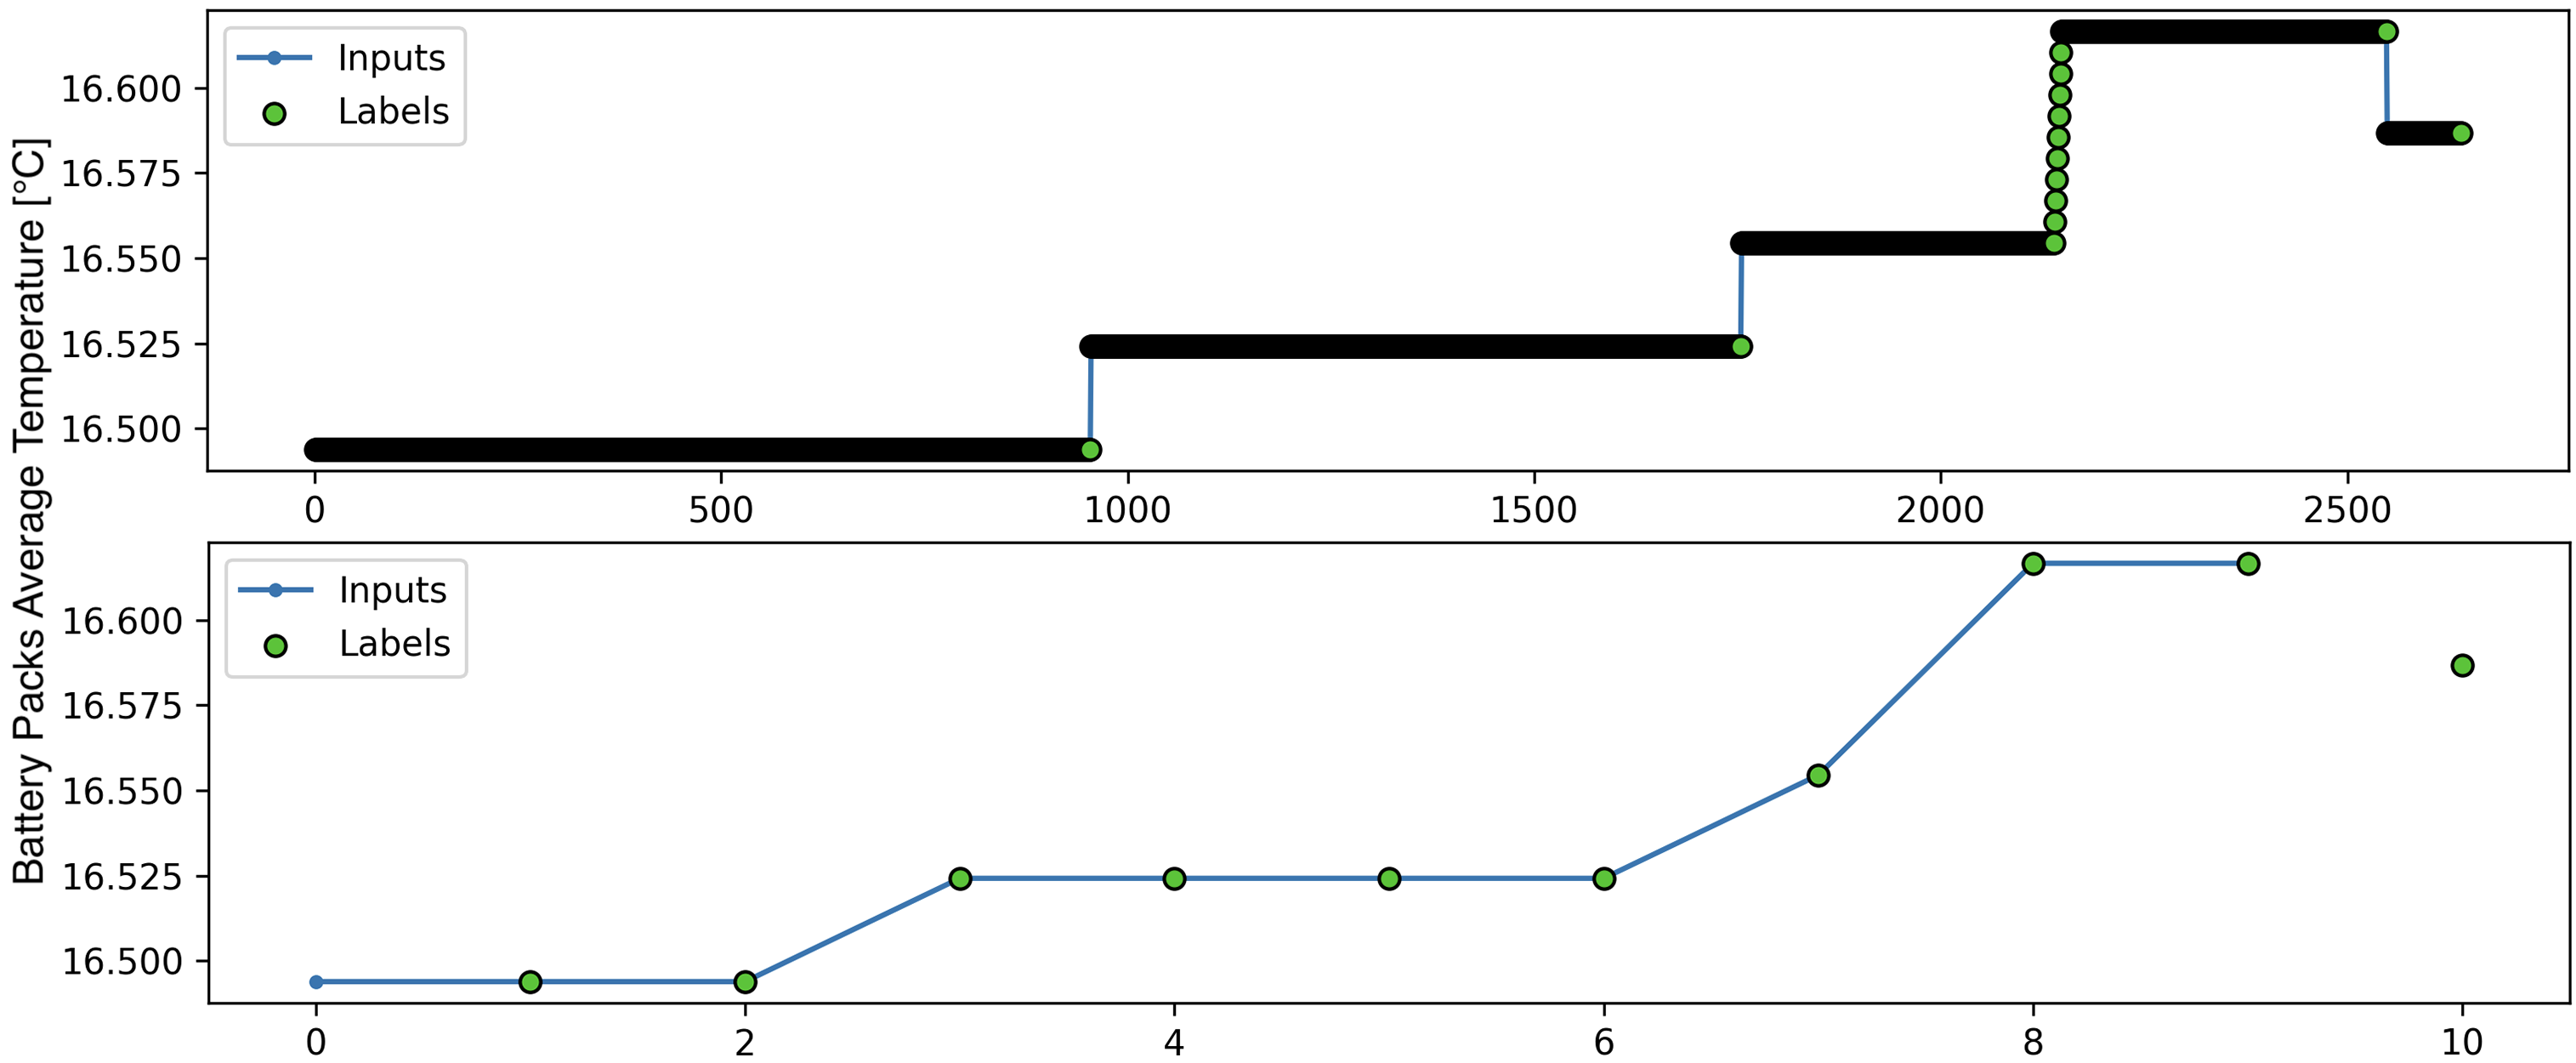
\includegraphics[width=\textwidth]{Chapter5/figures/data_sample2.png}
\caption{The temperature sample in 10 minutes}
\label{fig:temp_sample}
\end {center}
\end{figure}

On every trip, the value of these variables (i.e., accelerator pedal, braking pedal, speed, etc.) grows at the \gls{BEV} start-up as the extra features. 
From a training input point of view, a constant accumulation operation is closer to a battery's operating principle, a consequence of a chain reaction from driving manners. 
Also, Xu et al.~\cite{xu2021estimation} revealed that the discrete incremental capacity can improve the estimation accuracy of \gls{SOH}. 
Therefore, these features are processed to accumulate at the beginning of every trip. 

\subsubsection{Cyclical encoding}
the timestamp data is encoded into a cyclical representation of a particular day, season, and year with sine (\ref{eq:sine}) and cosine (\ref{eq:cosine})~\cite{petnehazi2019recurrent}. 
A total of six new cyclical features (i.e., day sine and cosine, season sine and cosine, year sine and cosine) have been added to emphasize the temperature climate for the \gls{ANN}. 

\begin{equation}
\label{eq:sine}
\text{Periodic sine} = \sin \left( \textit{timestamp}\times\frac{2\pi}{\textit{period}} \right)
\end{equation}

\begin{equation}
\label{eq:cosine}
\text{Periodic cosine} = \cos \left( \textit{timestamp}\times\frac{2\pi}{\textit{period}} \right)
\end{equation}
where:
\[
\text{period} = \begin{cases}
  \text{day} & 24 \times 60 \times 60\\
  \text{season} & 91.31 \times \textit{day} \\
  \text{year} & 365.24 \times \textit{day}
\end{cases}
\]

\subsection{Data windowing}
The input and output window size is set to 10 (i.e. 10 minutes). 
Summarised from the dataset, the average cool-down time for the entire battery pack is approximately 10 to 15 minutes at 1°C when driving. 
The output window size of 10 gives the driver sufficient time to ameliorate the driving behaviors or conditions for the drivers, which is intended to keep the battery pack's temperature in better condition. 

To enable the many-to-many predictions of the model, trip data is sliced into the size window for both the input and output for the model training. 
This consecutive windowing allows the model to predict the next $\mathit{x}$ minutes, based on the current $\mathit{x}$ minutes. 
The following Figure~\ref{fig:data_windowing} demonstrated the construction of ten-time steps of the input and output labels from the dataset. 
A shuffleable batch of input is generated by sliding the window for the next one-time step. 
The different \glspl{ANN} (e.g., linear network, \gls{LSTM}) are processed propinquity to satisfy the network input shape requirements. 
In general, the data is split into 70\% for training, 20\% for validation, and 10\% for testing for \gls{AI} model training. 

\begin{figure}[hbt]%[!ht]
\begin {center}
\begin{tikzpicture}[
array/.style={ 
                matrix of nodes,
                nodes={draw=black!80, minimum size=20, anchor=center},
                column sep=-\pgflinewidth,
                column 4/.style={nodes={draw=black!80, fill=gray!20}},
                column 5/.style={nodes={draw=black!80, fill=gray!20}},
                column 6/.style={nodes={draw=black!80, fill=gray!20}},
             },
dot/.style={fill,circle,inner sep=0pt,minimum size=3pt}             
]
\matrix[array] (array1) {
$t=1$ & $\cdots$ & $t=10$ & $t=11$ & $\cdots$ & $t=20$
\\};
\matrix[array, shift={(0.5,-1)}] (array2) {
$t=2$ & $\cdots$ & $t=11$ & $t=12$ & $\cdots$ & $t=21$ 
\\};
\matrix[array, shift={(1,-2)}] (array3) {
$t=3$ & $\cdots$ & $t=12$ & $t=13$ & $\cdots$ & $t=22$ 
\\};
\draw [ultra thick, 
    decorate, 
    decoration = {
                    calligraphic brace,
                    raise=5pt,
                    amplitude=5pt
                }] (-2.8,0.5) --  (-0.1,0.5)
node[pos=0.5,above=10pt,black]{$input$};                
\draw [ultra thick, 
    decorate, 
    decoration = {
                    calligraphic brace,
                    raise=5pt,
                    amplitude=5pt
                }] (-0.1,0.5) --  (2.8,0.5)
node[pos=0.5,above=10pt,black]{$label$};
\draw [ultra thick,
    black,
    decorate, 
    decoration = {
        calligraphic brace,
        raise=5pt,
        amplitude=5pt,
        }] (-3,-3.2) --  (-3,0.3)
node[pos=0.5,left=10pt,black]{$batch$};
\node[dot] (a) at (1.2,-2.8) {};
\node[dot] (a) at (1.28,-2.95) {};
\node[dot] (a) at (1.36,-3.10) {};
\end{tikzpicture}
\caption{The consecutive many-to-many window training input for Artificial Neural Network.}
\label{fig:data_windowing}
\end {center}
\end{figure}


\section{Charging and idling phases of the entire dataset}

The above dataset is extended to January 2023 with Odometer 22,500 kilometers of without drivers' label.
In this study, the \gls{SOH} values provided by \glspl{EV} are used as a reference to monitor battery performance. 
However, the lack of transparency surrounding the methodology employed by manufacturers to calculate these \gls{SOH} values introduces uncertainties. 
This opacity limits the reliability of the \gls{SOH} as an accurate indicator of battery health. 
Despite these challenges, a degree of predictability remains: as the intensity of electrical usage increases, a corresponding decline in \gls{SOH} is anticipated. 
Nevertheless, the manufacturer-provided \gls{SOH} metrics may not fully represent the nuanced and multifaceted nature of battery degradation over time.

% figure of SOH_join_A4.pdf
\begin{figure}[ht]
    \centering
    \includegraphics[width=\textwidth]{Chapter5/figures/SOH_join_A4.pdf}
    \caption{Battery health degradation in the \textit{Nissan Leaf}. (a) SOH decline by distance on the extended dataset. (b) Shift in peak charging voltage.}
    \label{fig:soh_odometer_charging_idling}
\end{figure}

Based on the insights gleaned from Figure~\ref{fig:soh_odometer_charging_idling}b, it's evident that the calendar effect on Li-ion batteries in real-world settings, especially during extended cycling, holds minimal if any significance. 
This observation leads to a pivotal realization: the genuine degradation of the battery pack is primarily linked to its discharge volume, particularly the energy withdrawn during usage.

To address this challenge, we've formulated an alternative method to gauge the authentic \gls{SOH}, leveraging the charging duration of \glspl{BEV} as a pivotal metric. 
As battery deterioration progresses over time, the available electric capacity within the battery decreases, manifesting in progressively shorter charging durations. 
The lower-left chart in Figure~\ref{fig:soh_odometer_charging_idling}b demonstrates the charging times of the Li-ion battery in the BEV across voltage ranges from 360 to 400 volts. 
A noticeable dip consistently emerges around 368 to 376 volts, corresponding to \gls{SOH} levels between 96\% to 91\%. 
Interestingly, this dip's characteristics exhibit a gradual rightward shift rather than a fixed voltage point exhibiting accelerated charging. 
By tracking this shifting pattern of the lowest peak, we can effectively discern the genuine trajectory of battery degradation. 
he observed voltage shifting pattern doesn't strictly adhere to a linear progression. 
Rather, the \gls{SOH} closely mirrors the trends evident in the vehicle's driving distance, as reflected by the odometer readings. 
This correlation suggests a robust link between driving patterns and battery degradation, opening the possibility for more precise predictions and the implementation of proactive maintenance strategies.

To overcome the limitations associated with the reliance on manufacturer-reported \gls{SOH} values, this study proposes an alternative approach. 
By focusing on the charging time of Battery \glspl{SOH}, a strong correlation between charging duration and battery degradation is revealed. 
As the battery's health deteriorates, its electric capacity diminishes, leading to a noticeable reduction in the time required for a full charge. 
This relationship provides a practical and observable metric for tracking battery health over time, offering a more transparent and operationally grounded perspective on degradation phenomena.

The analysis revealed a noteworthy correlation between driving distance and the degradation of the \gls{SOH} of the battery, as depicted in Figure~\ref{fig:soh_odometer_charging_idling}. 
This relationship underscores the cumulative impact of vehicle usage on battery health over time. 
Specifically, a 2.53\% decline in \gls{SOH} was observed as the driving distance increased from 5,000 km to 10,000 km. 
Beyond this range, the rate of \gls{SOH} degradation appeared to taper off, suggesting that the initial usage phase exerts a more pronounced effect on battery health compared to subsequent longer distances.

In addition to \gls{SOH} metrics, changes in charging behavior were also analyzed, revealing significant shifts in charging voltage and durations over the battery's lifecycle. 
Accelerated charging times were observed as the battery's capacity declined, providing an operational indicator of deterioration. 
These shifts align with the fundamental degradation mechanisms of lithium-ion batteries, where capacity loss leads to reduced energy throughput and faster charging completion times. 
Such trends further validate the use of charging profiles as a complementary measure for assessing battery health.

This analysis provides critical insights into the interplay between vehicle operation and battery degradation, emphasizing the importance of monitoring both usage patterns and charging behavior. 
By understanding these dynamics, it becomes possible to develop more effective battery management strategies and predictive maintenance schedules, ultimately enhancing the longevity and reliability of electric vehicle batteries.

By emphasizing the link between charging behavior and battery performance, this research not only sheds light on the inadequacies of current \gls{SOH} reporting but also provides a viable framework for monitoring and predicting battery health in real-world applications. 
This approach has the potential to enhance the understanding of degradation processes and contribute to the development of more accurate, user-friendly tools for \gls{EV} battery health management.


\section{Driving Behavior and Power Consumption}

The power consumption behavior of seven drivers (Drivers 1 through 7) was systematically analyzed, with a particular focus on the discharge phase when vehicle speeds exceeded 0 km/h. 
This detailed assessment offers insights into the individual driving patterns and their impact on energy consumption. As depicted in Figure~\ref{fig:consumption}, 
Drivers 1, 2, and 3 emerged as the primary contributors to the driving test in terms of overall distance covered, driving duration, and average speed. 
However, Driver 1 displayed a marginally lower driving distance compared to Drivers 2 and 3, despite a similar driving duration. 
This discrepancy may be attributable to unique characteristics of the road segments encountered, highlighting the need for further verification through \gls{GPS} data analysis.

% figure of consum_A4.pdf

\begin{figure}[ht]
    \centering
    \includegraphics[width=\textwidth]{Chapter5/figures/consum_A4.pdf}
    \caption{Overview of power consumption and influencing factors}
    \label{fig:consumption}
\end{figure}

To explore the factors influencing power consumption, critical variables such as air conditioning usage, the activation of \gls{ECO} mode, and the deployment of the ePedal system were examined. 
These factors were evaluated in terms of their effects, measured as hours of operation per kilometer driven. 
An intriguing finding was that Driver 5 exhibited the highest power consumption among all participants, even when utilizing \gls{ECO} mode and the ePedal system—features specifically designed to enhance energy efficiency. 
Additionally, Driver 5 demonstrated substantial regenerative power generation, creating a paradoxical scenario. 
This unusual pattern suggests complex interactions between regenerative braking, driving behavior, and environmental conditions, offering a unique opportunity to derive insights into optimizing energy consumption.

Through an in-depth examination of these driver profiles, this study seeks to uncover the underlying factors contributing to variations in energy consumption. 
Identifying these determinants is critical for formulating strategies aimed at improving the energy efficiency and overall performance of electric vehicles. 
By leveraging such insights, the findings can support the development of tailored recommendations for drivers and manufacturers, fostering advancements in sustainable mobility and the operational optimization of electric vehicle systems.

A detailed correlation coefficient test is performed on the \gls{SOH} data to find out the cause of the sharp decline. 
In particular, the high temperature of the battery pack due to the driving style and seasons. 
Table~\ref{table:soh} resumes few critical variables: the \gls{HV} battery voltage and current, \gls{SOC}, and pack temperature are ranked at the bottom of the list. 
From a statistical perspective, the degradation of the battery can not be simply revealed. 


\begin{table}[!ht]
\centering
\caption{Top 10 degradation variables correlated to SOH}
\begin{tabular}{c|cl|cl}
    \label{table:soh}
    Ranking & Pearson &  & Spearman \\
    \hline
    1 & -0.955 & Timestamp          & -0.998  & Timestamp          \\
    2 & -0.517 & ECO                & -0.998  & Odometer           \\
    3 & -0.445 & Charge Mode        & +0.897  & Ah                \\
    4 & +0.358 & Ah                 & -0.365  & Charge Mode        \\
    5 & -0.344 & Nissan ePedal      & -0.350  & Plug State          \\
    6 & -0.231 & Battery Voltage    & -0.323  & ECO mode            \\
    7 & +0.224 & RPM                & +0.285  & Motor Temp.         \\
    8 & -0.193 & SOC                & -0.268  & ePedal             \\
    9 & +0.190 & Speed              & +0.209  & Pack4 Temp.         \\
    10 & -0.186 & HorsePower        & -0.207  & Battery Current     \\
    \hline
\end{tabular}

\begin{tablenotes}
  \small
  \item + same trend / - reverse trend
\end{tablenotes}
\end{table}

\section{Driving Behavior and Battery Thermal Conditions}

This section categorizes driving styles and examines their thermal effects:

\begin{itemize}
    \item \textbf{Gentle Driving:} Smooth accelerations and decelerations kept battery temperatures within the optimal range (15°C–35°C), minimizing stress on the battery and maintaining efficiency.
    \item \textbf{Aggressive Driving:} Sharp accelerations and frequent braking led to temperature surges exceeding 41°C, particularly in high ambient temperatures, imposing additional thermal stress on the battery.
    \item \textbf{Cautious Driving:} Minimal pedal input was typical, but during winter conditions, prolonged exposure to suboptimal temperatures (<15°C) resulted in efficiency losses and potential risks to long-term performance.
\end{itemize}

Established that driving out of the optimal temperature range affects the battery capacity significantly, the \gls{SOH} loss happened even in normal conditions. 
Thus, there could be other influencing factors that have an impact on \gls{SOH}. 
The driving style is considered and investigated, in correlation with the car speed, horsepower (calculated by (\ref{eq:horsepower})), temperature, pressure on the pedal, among different drivers (i.e. gentle, aggressive, and caution). 
The Figure~\ref{fig:all_driving_status} [a] revealed the overall status. 

\begin{equation} \label{eq:horsepower}
    \textrm{Horsepower}\footnote{We used mechanical horsepower where 1 kW = 1.3410220888 hp(I)} = 1.341\times\left((Voltage \times Current)/1000)\right)
    \end{equation}

\begin{figure*}[hbt]
    \includegraphics[width=\textwidth]{Chapter5/figures/plotly_titles.png}
    \caption{Battery temperature status on different driving styles}
    \label{fig:all_driving_status}
\end{figure*}

Six drivers participated in the test period. 
Despite all the drivers run averagely in optimal temperature range (Figure~\ref{fig:all_driving_status}[b]). 
The driving styles of drivers \#1 and \#4 raised the battery temperature from 35°C to 41°C (Figure~\ref{fig:all_driving_status}[c]). 
Drivers \#1, \#2, \#5, and \#6 encountered a low battery temperature (15°C to 6°C) during the vehicle startup in winter (Figure~\ref{fig:all_driving_status}[d]). 
To clarify specific aspects of the different diving styles, October 2021 (the last full month) is selected for a detailed comparison. 
The average ambient temperature was 16.48°C, and the 25\% to 75\% range is depicted in blue in Figure~\ref{fig:all_driving_status} [e] by ignoring the trip distance, duration, and road type. 
Driver \#1 is the only one who could push the battery temperature above 35°C. 
However, the mean and median of the speed and horsepower of driver \#1 were not the highest (Figure~\ref{fig:all_driving_status} [f,g]). 
Instead, the pressure on the braking pedal was the highest among all drivers. 
This implies that the braking style or the regenerative braking may have aggravated the battery overheating. 

\begin{figure}[hbt]%[!ht]
    \begin {center}
    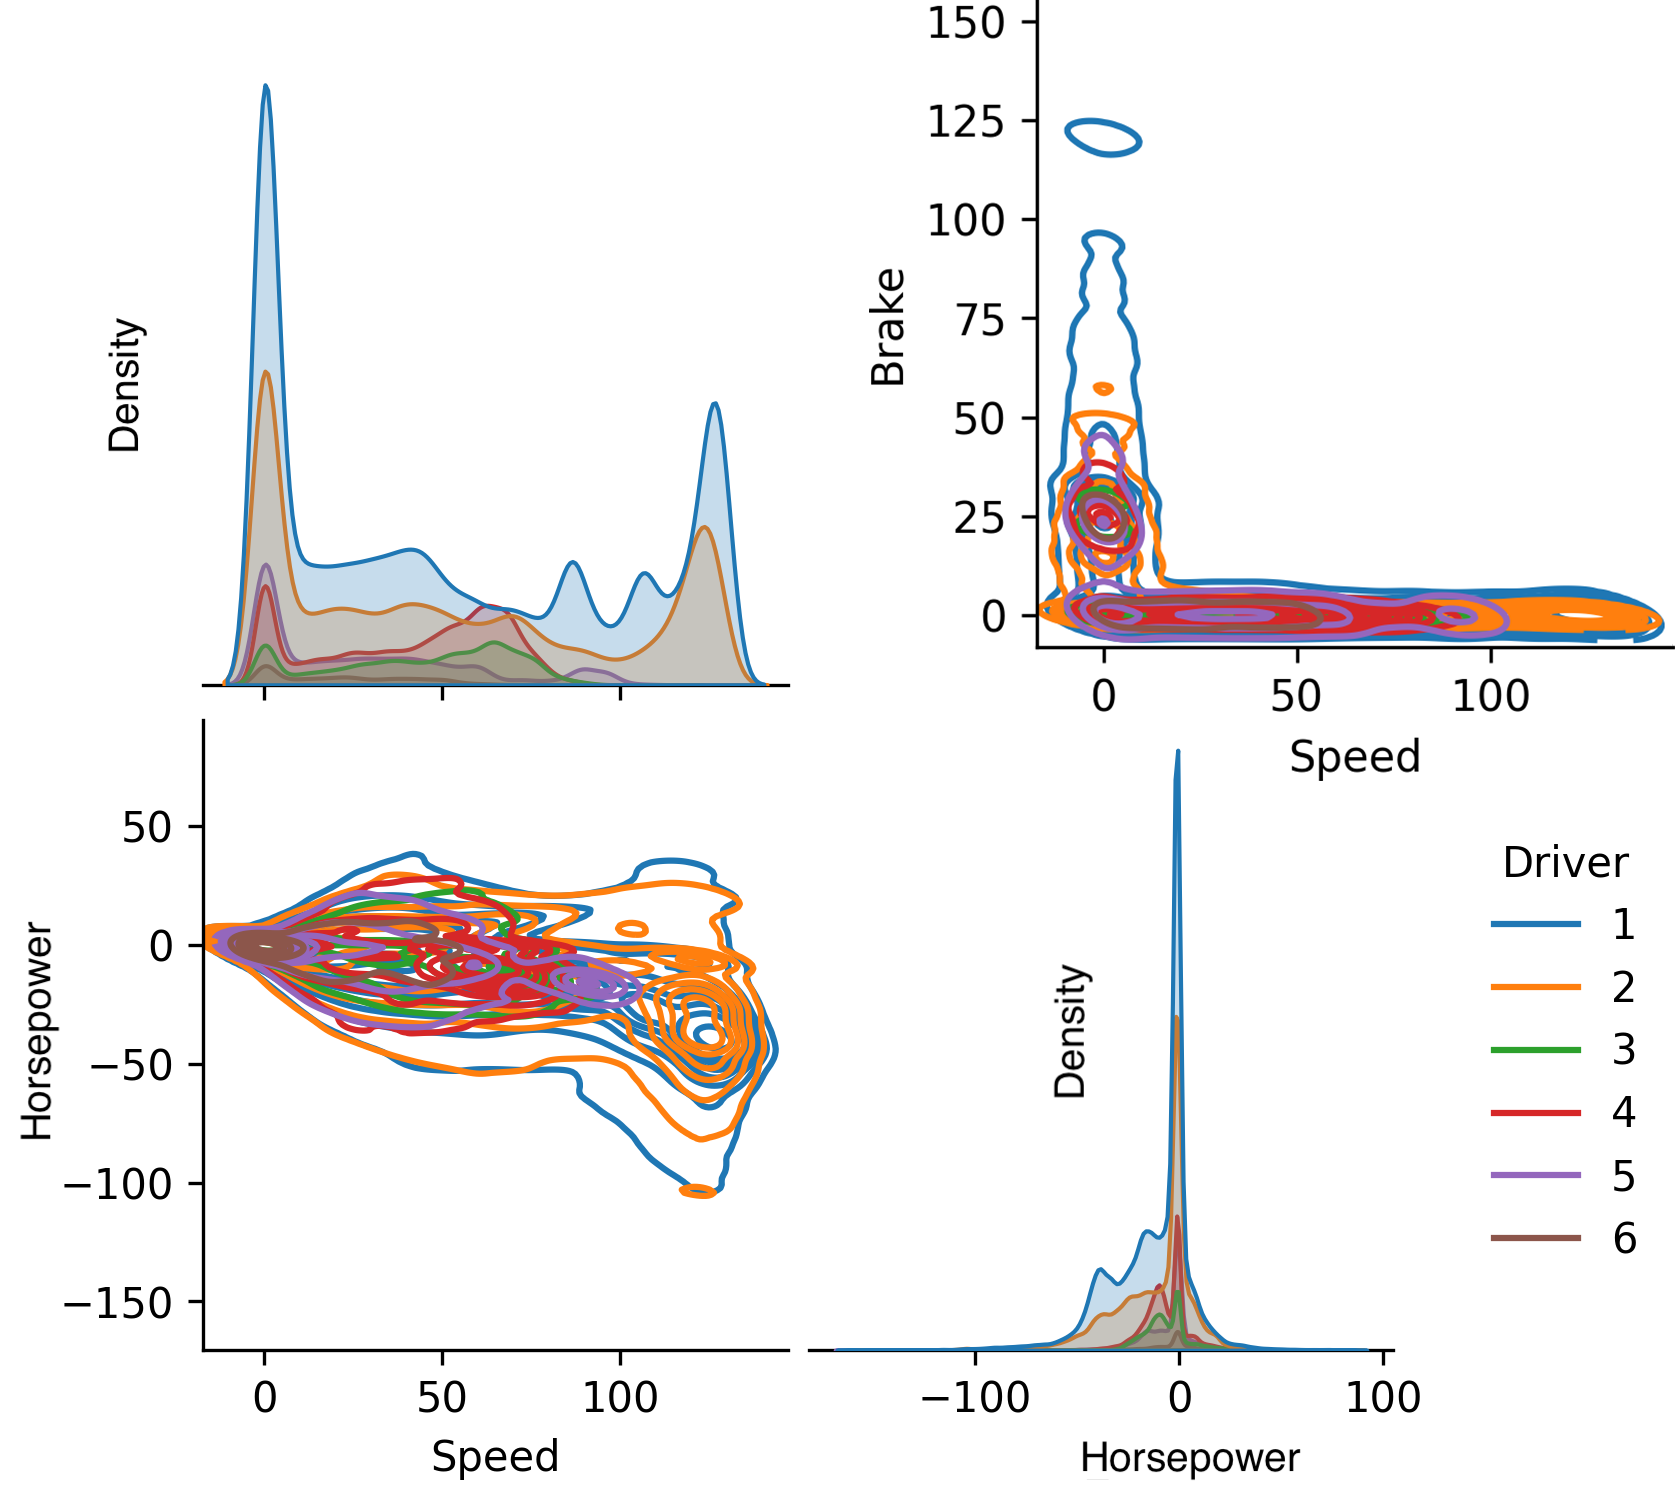
\includegraphics[width=0.75\textwidth]{Chapter5/figures/power_band_density.png}
    \caption{Power band of the \textit{Nissan Leaf} at different speed}
    \label{fig:power_band}
    \end {center}
\end{figure}

Figure~\ref{fig:power_band} shows the speed and horsepower kernel density estimation for all the drivers. 
A good driving operation from the battery perspective should have a smooth horsepower output and a lower braking force. 
However, driver \#1 had an enormous bandwidth fluctuation at the horsepower density and the brake. 
Although the mean of the horsepower of driver \#1 was not the highest. 
Combining with the battery pack temperature overheating shown in Figure~\ref{fig:all_driving_status} [e], we can conclude that driver \#1 was the most aggressive. 

Table~\ref{table:good_driving_style} summarizes the speed, acceleration pedal pressure, brake pressure, and horsepower to expose the proper driving behaviors with a \textit{Nissan Leaf}, to maintain the battery pack's best thermal condition (15°C to 35°C). 
A pleasing driving style across the different speeds needs to control: 
\textbf{(1)} the acceleration rate of speed smoothly and linearly with less standard deviation, especially at high speed (std. less than 6 km/h); 
\textbf{(2)} the acceleration pedal pressure at approximately 17/43/26/45 under the speed of 50/90/110/130 km/h; 
\textbf{(3)} the brake at low pressure at high speed and average pressure of 7 at low speed. 
Also, reduce the frequent braking. The higher the speed, the less the braking; 
\textbf{(4)} the horsepower at the average of -3/-12/-22/-34 kW corresponding to the speed of 50/90/110/130 km/h if that is visible to the driver. 
\textbf{(5)} the acceleration and braking forces on the pedals stay as smooth as possible at the winter startup. 

\begin{table}[!ht]
    \centering
    \caption{Good driving style}
        \begin{tabular}{l|c|c|c|c}
        \label{table:good_driving_style}
        ~ & Speed [km/h] & Acc. pedal & Brake pedal & Horsepower [kW]\\ \hline
        ~ & \multicolumn{4}{c}{\multirow{2}{*}{City towns [50km/h]}} \\\\ \hline
        Mean & 13.10 & 16.62 & 7.00 & -3.19\\
        Std. & 16.55 & 24.95 & 16.04 &9.60\\ \hline
        ~ & \multicolumn{4}{c}{\multirow{2}{*}{Single carriageways [90 km/h]}} \\\\ \hline
        Mean & 67.43 & 43.14 & 0.38 & -11.50\\
        Std. & 11.46 & 32.81 & 2.88 & 18.25\\ \hline
        ~ & \multicolumn{4}{c}{\multirow{2}{*}{Dual carriageways [110 km/h]}} \\\\ \hline
        Mean & 100.82 & 26.31 & 0.14 & -22.00\\
        Std. & 5.98 & 38.24 & 1.94 & 23.56\\ \hline
        ~ & \multicolumn{4}{c}{\multirow{2}{*}{Motorways [130 km/h]}} \\\\ \hline
        Mean & 123.05 & 45.41 & 0.06 & -34.40\\
        Std. & 5.09 & 49.03 & 1.03 & 21.56\\
        \hline
        \end{tabular}
\end{table}

Illustrating from the data, battery life could be enhanced by evaluating the actual temperature on the pack and making the corresponding improvements at driving style to slow down the degradation. 
Aggressive driving manners could speed up battery degradation due to the temperature variation, which usually results from rough handling or improper pedal use. 
Also, the seasonal temperature shown in Figure~\ref{fig:seasonal_temp} is the main influencing factor on the battery pack's temperature when driving \glspl{EV}.

\section{Bidirectional Long Short-Term Memory Model for Temperature Prediction}
To predict battery pack temperature under varying conditions, a \gls{Bi-LSTM} model was developed. The architecture and training process are described below:

\subsection{Model Architecture}

The LSTM model is built in favor of simplicity because of lesser features and reprocessed. 
Also, the battery temperature prediction tends to perform better in the simple model with less past status by the temperature characteristic~\cite{fang-2012,jaliliantabar2022prediction}. 
In the model evaluation, the \gls{MAE} (\ref{eq:mae}) is adopted. 
To prevent overfitting of simple machine learning models, L2 regularization (\ref{eq:l2}) is added into the \gls{MSE} loss function to penalize models. 

\begin{equation}
\label{eq:mse}
    \text{MSE}=\frac{1}{n}\sum_{i=1}^{n}(\mathit{y_{i,t}-y_{i,p}})^2
\end{equation}
\begin{equation}
    \label{eq:mae}
    \text{MAE}=\frac{1}{n}\sum_{i=1}^{n}|\mathit{y_{i,t}-y_{i,p}}|
\end{equation}
\begin{equation}
\label{eq:l2}
\text{L2}=\lambda \sum_{i=1}^{n}\mathit{w_i}^{2}
\end{equation}
Where the $y_{i,t}$, $y_{i,p}$, and $n$ are target value, predicted value, and number of samples in the dataset.


\subsection{Training Process}

To construct the network and hyperparameter tuning, Optuna is adopted. 
It is a neural network optimization framework that automates the searching and pruning strategy for different networks~\cite{optuna_2019}. 
Compared to the grid search and random search, Optuna can reduce the computational resources significantly and better locate the minima. 
Figure~\ref{fig:optuna} shows the overall structure of the Optuna. 
Firstly, the three dimension input is reshaped into the batch and the vector of window size times features as the input to the Optuna. 
The Optuna framework then searches automatically for the best number of layers, neurons, and regularization for the intermediate network. 
A \gls{FC} layer is attached after Optuna to convert the different network settings to a constant shape. 
Finally, the \gls{FC} layer is reshaped to the output window shape. 

\begin{figure}[hbt]%[!ht]
\begin {center}
\begin{tikzpicture}[%
    >=triangle 60,              % Nice arrows; your taste may be different
    start chain=going below,    % General flow is top-to-bottom
    node distance=4mm and 38mm, % Global setup of box spacing
    every join/.style={norm},   % Default linetype for connecting boxes
    ]
% ------------------------------------------------- 
% A few box styles 
% <on chain> *and* <on grid> reduce the need for manual relative
% positioning of nodes
\tikzset{
  base/.style={draw, on chain, on grid, align=center, minimum height=2ex},
  proc/.style={base, rectangle, text width=8em},
  test/.style={base, diamond, aspect=2, text width=5em},
  term/.style={proc, rounded corners},
  % coord node style is used for placing corners of connecting lines
  coord/.style={coordinate, on chain, on grid, node distance=6mm and 25mm},
  % nmark node style is used for coordinate debugging marks
  nmark/.style={draw, cyan, circle, font={\sffamily\bfseries}},
  % -------------------------------------------------
  % Connector line styles for different parts of the diagram
  conb/.style={->, draw},
  norm/.style={->, draw},
  free/.style={->, draw},
  cong/.style={->, draw},
  it/.style={font={\small\itshape}}
}
% -------------------------------------------------
\node [proc] (p1) {Window input};
\node[left=1mm of p1] {[b, w, f]};
\node [proc, join=by conb] (p2) {Reshape};
\node[left=1mm of p2] {[b, w*f]};
\node [proc, fill=gray!20, join=by conb] (p3) {Optuna};
\node [proc, join=by conb] (p4) {FC layer};
\node[left=1mm of p4] {[b, w*f]};
\node [proc, join=by conb] (p5) {Reshape ouput};
\node[left=1mm of p5] {[b, w, f]};
\node[proc, fill=gray!20, right=of p3] (p6) {
    Layers\\
    Neurons\\
    Optimizer\\
    Learning rate\\
    Regularization 
};
\draw [dashed, line width=0.2mm] (p3.north east) -- (p6.north west);
\draw [dashed, line width=0.2mm] (p3.south east) -- (p6.south west);
\node[font=\footnotesize, below=1mm of p6] (explain) {
    \begin{tabular}{ll}
    b: & batch \\
    w: & window size \\
    f: & features 
    \end{tabular}
};
\end{tikzpicture}
\caption{Optuna framework structure for automatic search and network construction.}
\label{fig:optuna}
\end {center}
\end{figure}

Table~\ref{tab:optuna_settings} shows the detailed searching parameters setting inside the Optuna layers. 
The activation and initialization are fixed to Relu and He uniform variance to reduce the searching time. 
The search of hyperparameter combinations is set to 1,000 for the model. 
The following Table~\ref{tab:bestmodel} shows the settings of our best model.

\begin{table}[hbt]
    \centering
    \caption{Hyperparameter Searching and Best Model Settings}
    \label{tab:combined_tables}
    \begin{minipage}[t][6cm][t]{\textwidth} % Make Table A bigger
        \centering
        \subcaption{The Optuna Automatic Search Settings}
        \label{tab:optuna_settings}
        \begin{tabular}{@{}ll@{}}
            \toprule
            Optuna & Settings \\ \midrule
            Max. searches & 1,000 \\
            Max. layers & 10 \\ 
            Neurons & 4 to 512 \\ 
            Optimizer & Adam, SGD, RMSProp \\ 
            Learning rate & 1e-5 to 1e-1 \\ 
            Regularization & 1e-10 to 1e-3 \\
            \bottomrule
        \end{tabular}
    \end{minipage}
    \hfill
    \begin{minipage}[t][6cm][t]{\textwidth} % Make Table B smaller
        \centering
        \subcaption{The Best Model - Bidirectional LSTM}
        \label{tab:bestmodel}
        \begin{tabular}{@{}ll@{}}
            \toprule
             & Settings \\ \midrule
            Layers & 3 \\
            Structure & Bi-LSTM(341) x Bi-LSTM(32) x FC(420) \\ 
            Optimizer & Adam \\ 
            Learning rate & 6.48E-05 \\ 
            Regularization & 1.33E-10 \\
            Early stopping & with validation loss \\
            Total parameters & 1,257,892 \\
            \bottomrule
        \end{tabular}
    \end{minipage}
\end{table}


\section{Results}\label{sec:result}

In this section, the results and implications of our best model are presented. 
The different datasets and models are compared to identify the most important factors for temperature prediction. 
The ablation study on the features was also included to verify the importance of feature engineering. 
The limitations and considerations of our work are also discussed. 
Finally, the consequences of the capacity loss caused by temperature are explained. 

\subsection{Justification of the best model}

The MAE on the prediction of the average temperature of the battery pack is the performance indicator for all models. 
Table~\ref{tab:top_models_settings} shows the different model comparisons using the test data (10\%) and a 10-fold cross-validation. 
Two output variables are tested that are associated with the constant input of 10 window steps: 
(i) the output of 10 temperature predictions (10 minutes) which is our main goal; 
(ii) the output of a single temperature prediction in the last minutes of the 10 minutes as a reference. 

\begin{table}[hbt]
    \centering
    \caption{The MAE benchmarking [°C]}
    \label{tab:top_models_settings}
    \begin{tabular}{lcccc}
    \toprule
        Models & 10 Predictions & 10-Fold-10 & 1 Prediction & 10-Fold-1 \\ 
        \midrule
        \gls{CNN} & 7.69 & 7.36 & - & - \\ 
        \gls{MLP} & 7.69 & 7.35 & 7.9 & 7.33 \\ 
        Linear & 13.2 & 12.16 & 14.74 & 13.29 \\ 
        \gls{LSTM} & 3.16 & 2.12 & 4.14 & 3.21 \\
        \gls{Bi-LSTM} & 2.92 & 1.7 & 2.83 & 2.06 \\ 
    \bottomrule
    \end{tabular}
\end{table}

The \gls{Bi-LSTM} model showed the smallest error of 2.92°C in the test data and a mean error of 1.7°C in the cross-validation of the 10 predictions output. 
When these two errors are averaged, an error of 2.31°C is the best performance we found for this model. 
The multi-window linear model showed the worst performance among the models. 
There is almost no difference in the prediction errors between the \gls{CNN} and \gls{MLP} models. For reference, the model with one output shows similar performance. 
The \gls{CNN} model is not available for single output due to the restriction to a minimum dimension. 

\begin{figure}[hbt]%[!ht]
\begin {center}
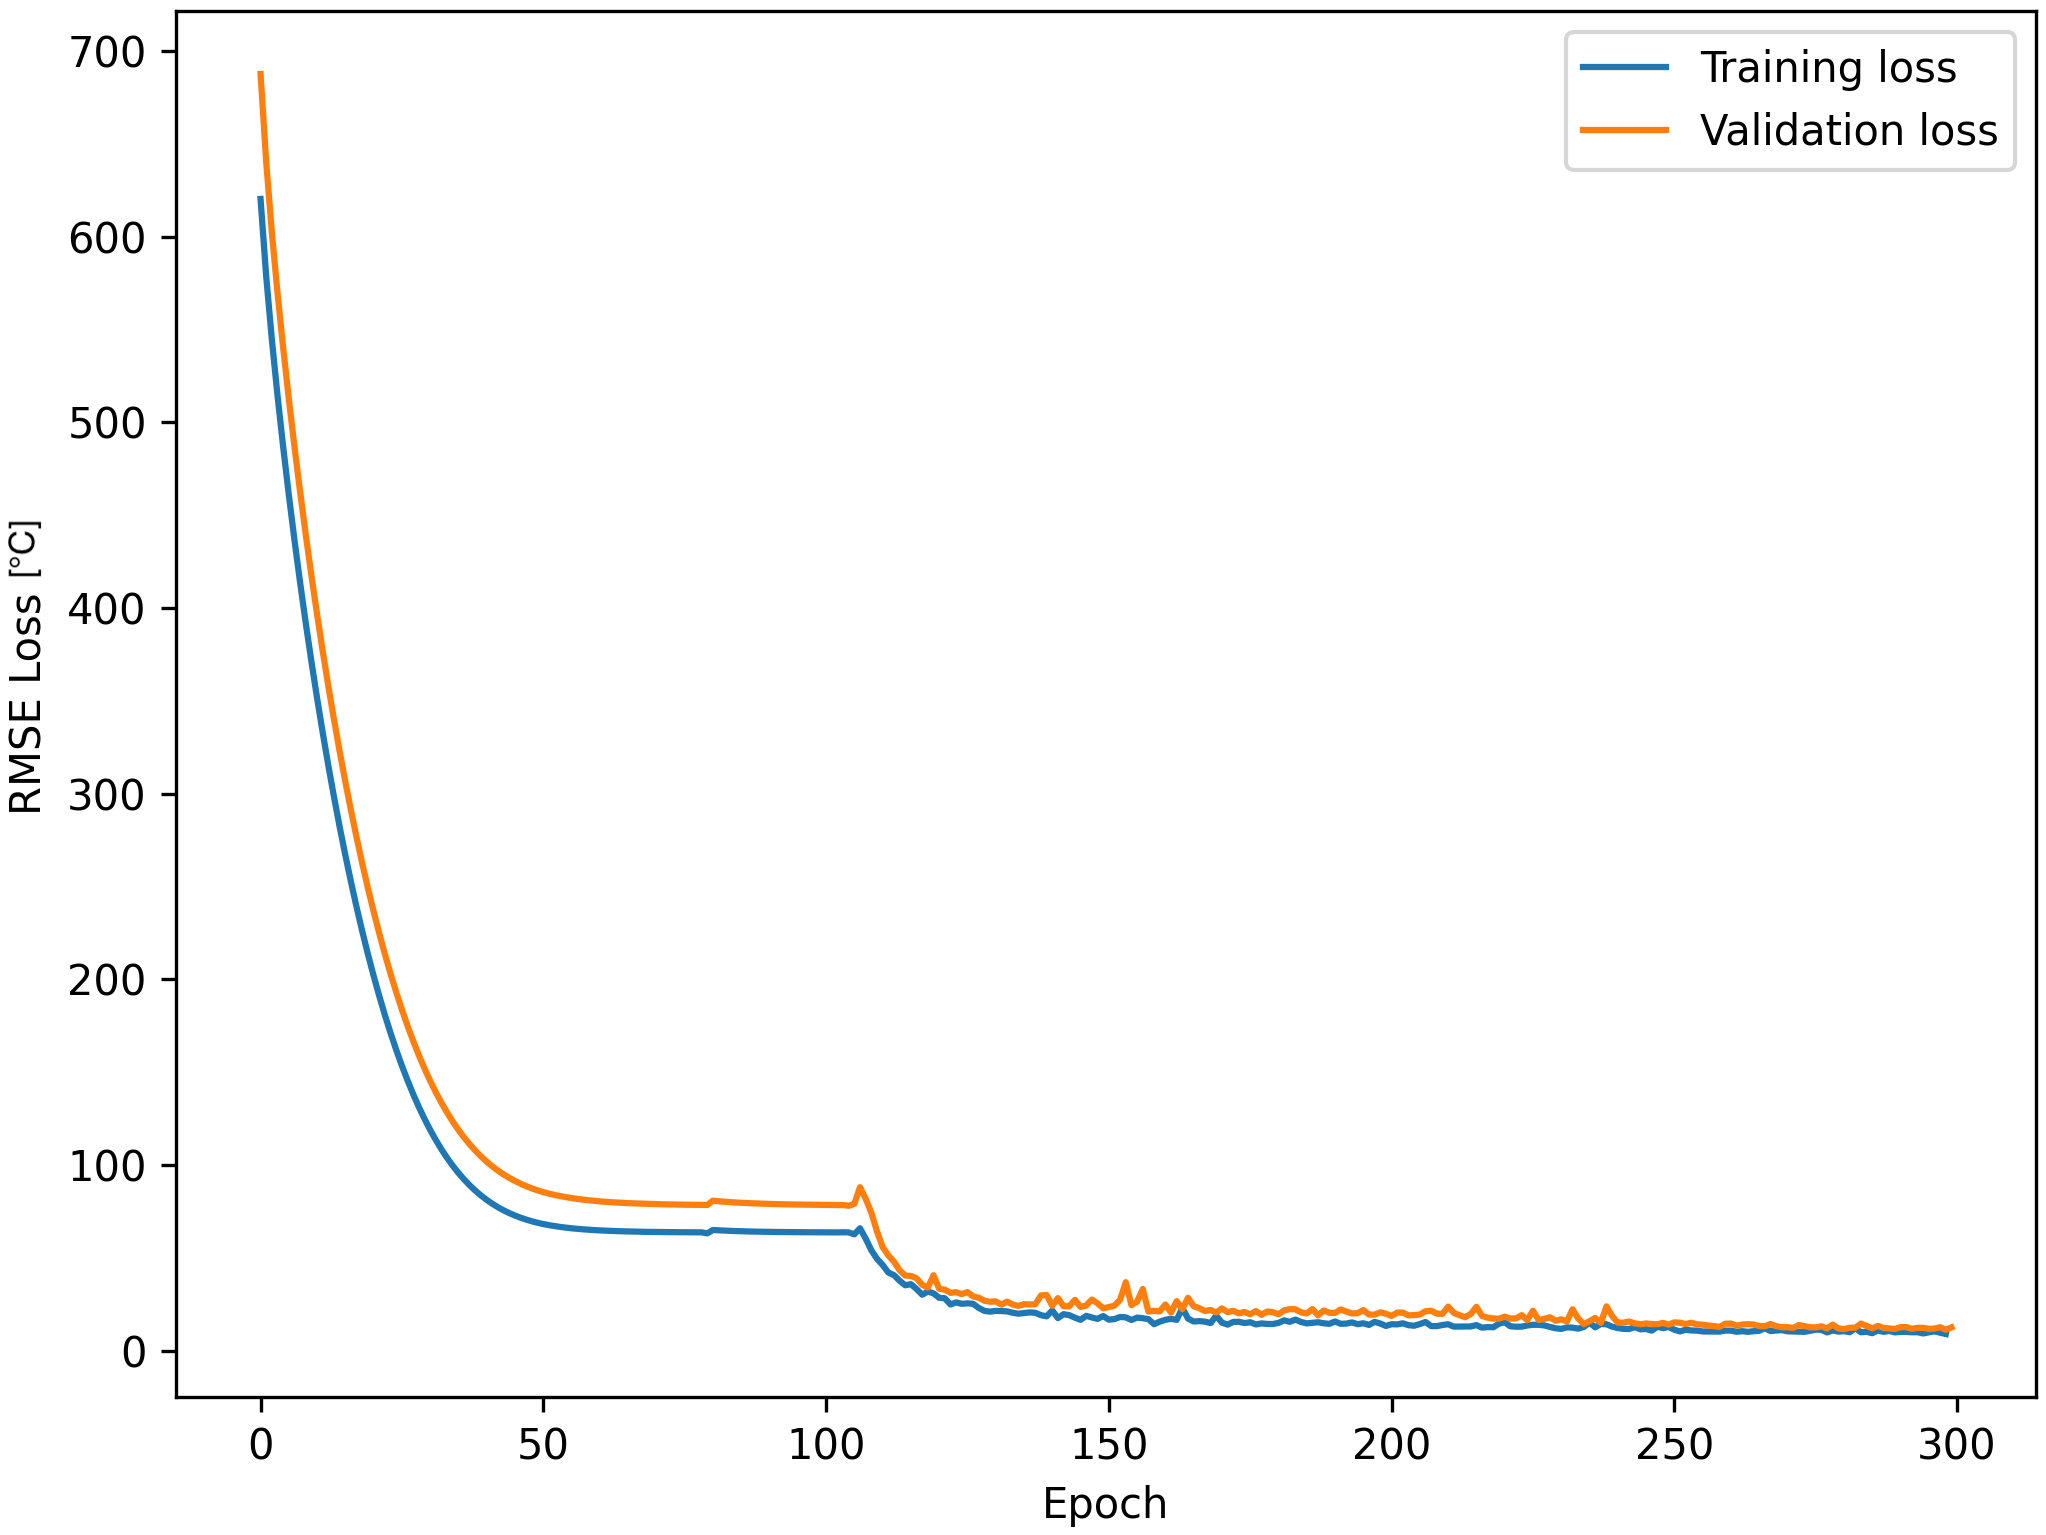
\includegraphics[width=0.8\textwidth]{Chapter5/figures/lstm_loss_nodriver_temp.png}
\caption{Training loss on the best model}
\label{fig:lstm_loss}
\end {center}
\end{figure}

The training and validation loss is shown in Fig.~\ref{fig:lstm_loss}. 
The training of the model converges smoothly in the first 300 epochs with a time cost of about 2,400 seconds. 
The validation loss of the model gradually decreases and overlaps with the training loss at epoch 250.

\subsection{Ablation study}

The ablation study focuses on the features, as Optuna had sought the optimal structure for the model, which is a standard model without adjustments. 
Table~\ref{tab:ablation} shows the result of removing accumulated variables, time signals, both accumulated variables and time signals, and trip labels.

\begin{table}[hbt]
    \centering
    \caption{The \gls{MAE} on features ablation}
    \label{tab:ablation}
    \begin{tabular}{lcc}
    \toprule
        Remove & \gls{MAE} [°C] & 10-Fold-10 [°C]\\ 
        \midrule
        Accumulated features & 7.69 & 7.36 \\ 
        Time & 3.87 & 3.87 \\ 
        Accumulated features and Time & 7.69 & 7.36 \\
        Trip label & 3.5 & 3.29 \\
        \bottomrule
    \end{tabular}
\end{table}

We have found that the accumulated characteristics are of significant importance. 
When removed, the \gls{MAE} increases to 7.69°C. This shows that the Bi-LSTM model is partially based on the linear signal.
When the time signal is removed, the \gls{MAE} of the model increases by about 1°C. 
Based on the model results, temporal variations (e.g., seasonal factors or road conditions) also affect the temperature of the battery pack. 
Finally, the temperature increases by about 0.6°C when a trip number is removed. 
In addition, we recorded an \gls{MAE} increase to 4.41°C and a 10-fold validation of 2.17°C when adding the driver ID as a feature.

\subsection{Dataset comparison}

To our knowledge, this is the only dataset collected without simulation or modeling on a real \textit{Nissan Leaf's} \gls{ECU}. 
Instead of comparing the model to the existing dataset, we compare it to the new dataset assembled from our data. 
It is because the above feature ablation study shows the importance of features. 
Also, it may not be comprehensive enough to compare performance with the different battery types, cells, and laboratory-tested datasets~\cite{DOSREIS2021100081}. 
This resampled dataset follows China's mandatory electric vehicle data collection protocol \href{https://openstd.samr.gov.cn/bzgk/gb/newGbInfo?hcno=674DE45C0AD3DE2CD75B9C4CD8ED57C1}{GB/T 32960.3} and our feature engineering steps. 
The difference between the GB/T 32960 dataset and ours is the sampling rate of 30 seconds.

\begin{table}[hbt]
    \centering
    \caption{The \gls{MAE} difference on the Chinese standard}
    \label{tab:gbt32960}
    \begin{tabular}{lcc}
    \toprule
        Dataset & \gls{MAE} [°C] & 10-Fold-10 [°C] \\ 
        \midrule
        30s resampled & 3.57 & 1.76 \\ 
        Ours & 2.92 & 1.7 \\ 
        \midrule
        Difference & 0.65 & 0.06 \\
        \bottomrule
    \end{tabular}
\end{table}

Table~\ref{tab:gbt32960} shows a very small loss of precision in both \gls{MAE} and 10-fold validation when predicting 10 outputs. 
Compared to our 250ms fine-time granularity, the Bi-LSTM model still performs effectively at the 30s interval for temperature prediction on the battery pack.

\subsection{Statistical learning comparison}

To understand the performance of our data, statistical learning models are compared. 
Four one-to-one models, including \gls{SVR} with Gaussian kernel, linear, Ada Boost Regressor and Decision Tree Regressor, are implemented to test the prediction errors. 
The ratio of training and testing is set to 0.67 and 0.33, respectively. 
Table~\ref{tab:stat_learning} shows that the linear model achieves the minimum MAE error of 0.41°C. 
However, this result cannot be directly compared with our model because it cannot detect the input in the next $\mathit{x}$ minutes.

\begin{table}[hbt]
    \centering
    \caption{The \gls{MAE} of the statistical learning approach}
    \label{tab:stat_learning}
    \begin{center}
    \begin{tabular}{ll}
    \toprule
        Models & \gls{MAE} [°C] \\
        \midrule
        \gls{SVR}-Gaussian & 6.0258 \\ 
        Linear & 0.4058 \\ 
        Ada Boost Regressor & 0.612 \\ 
        Decision Tree Regressor & 0.8109 \\ 
    \bottomrule
    \end{tabular}
    \end{center}
\end{table}

\section{Discussion}

This study has provided a comprehensive examination of the interactions between driving behaviors, environmental conditions, and the thermal dynamics of \gls{EV} batteries. 
By utilizing a robust dataset and employing advanced \gls{ML} techniques, particularly the Bidirectional Long Short-Term Memory (\gls{Bi-LSTM}) model, this work has elucidated key factors impacting battery performance and degradation. 
The findings have significant implications for optimizing \gls{EV} battery management and extending operational lifespan.

\begin{itemize}

\item \textbf{Driving Behavior and Thermal Dynamics:}
The results demonstrate that driving behaviors significantly influence battery thermal conditions and State of Health (\gls{SOH}). 
Aggressive driving styles, such as frequent accelerations and sharp braking, were found to induce temperature surges exceeding 41°C, leading to thermal stress and accelerated \gls{SOH} degradation. 
Conversely, gentle driving styles maintained battery temperatures within the optimal range (15°C–35°C), mitigating thermal stress and preserving battery longevity.

\item \textbf{Environmental Impact:}
Seasonal and ambient temperature variations played a critical role in battery performance. 
Prolonged exposure to cold conditions (<15°C) during winter led to reduced energy efficiency and potential risks to long-term performance. 
High ambient temperatures in summer exacerbated thermal stress, particularly in aggressive driving scenarios, underscoring the importance of adaptive thermal management.

\item \textbf{Battery Degradation Metrics:}
The study highlighted the limitations of manufacturer reported \gls{SOH} metrics due to opaque methodologies. 
An alternative approach using charging duration as a degradation metric was proposed, revealing strong correlations between charging profiles and \gls{SOH}. 
This framework provides a practical method for monitoring battery health over time.

\item \textbf{Energy Efficiency and Driving Optimization:}
The investigation into power consumption uncovered significant inter-driver variability. 
Factors such as ePedal usage, \gls{ECO} mode activation, and regenerative braking exhibited varied effectiveness across drivers, suggesting the potential for personalized recommendations to optimize energy efficiency and driving performance.

\item \textbf{Model Performance and Predictive Accuracy:}
The \gls{Bi-LSTM} model achieved superior predictive accuracy with a mean absolute error (\gls{MAE}) of 2.92°C, outperforming other models. 
Feature engineering, including the incorporation of temporal signals and accumulated variables, proved crucial for improving prediction accuracy, demonstrating the efficacy of the model in handling complex real-world datasets.

\item \textbf{Practical Applications and Future Research:}
    \begin{itemize}
        \item \textbf{Predictive Maintenance:} Insights from this study can facilitate the development of predictive maintenance strategies, ensuring timely interventions to reduce battery degradation. 
        This approach is especially relevant for fleet management and high-utilization \gls{EV} scenarios.
        \item \textbf{Driver Behavior Optimization:} The findings highlight the importance of educating drivers on energy-efficient driving behaviors, such as smooth acceleration and minimizing braking, to enhance battery performance and longevity.
        \item \textbf{Advancements in Battery Management Systems:} Integrating data-driven insights into \glspl{BMS} can enable real-time adaptation to varying driving and environmental conditions, improving system reliability and safety.
        \item \textbf{Policy Implications:} Policymakers can use these findings to establish transparent standards for \gls{SOH} reporting and battery thermal management, benefiting both consumers and manufacturers.
    \end{itemize}

\item \textbf{Limitations and Research Recommendations:}
    \begin{itemize}
        \item The findings are primarily based on a specific \gls{EV} model (\textit{Nissan Leaf}) and may not generalize across different models or battery chemistries. 
        Expanding the analysis to other \gls{EV} platforms is recommended.
        \item Real-world data introduces variability that may obscure controlled experimental effects. Incorporating laboratory-controlled data could further validate the findings.
        \item The study's temporal scope limits the understanding of long-term battery degradation. 
        Extended longitudinal studies are necessary to explore the cumulative effects of usage on battery health.
    \end{itemize}

\end{itemize}

In conclusion, this study advances the understanding of the complex interactions between driving behaviors, environmental conditions, and battery thermal dynamics in \glspl{EV}. 
By leveraging advanced machine learning models and robust feature engineering, the proposed framework offers actionable insights into battery management and predictive maintenance. 
Addressing the identified limitations in future studies will contribute to the development of more efficient and sustainable electric vehicle technologies.

\endinput